\documentclass[12pt,a5paper]{article}
\usepackage[margin=.5in]{geometry}
\usepackage[utf8]{inputenc}
\usepackage[IL2]{fontenc}
\usepackage[czech]{babel}
\usepackage{microtype}
\usepackage{amssymb}
\usepackage{amsthm}
\usepackage{amsmath}
\usepackage{xcolor}
\usepackage{graphicx}

\usepackage[inline]{enumitem}

\newcommand{\R}{\mathbb{R}}

\setlist[enumerate]{label={(\alph*)},topsep=\smallskipamount,noitemsep}
\setlist[itemize]{topsep=\smallskipamount,noitemsep}

\theoremstyle{definition}
\newtheorem{uloha}{Úloha}
\newtheorem*{bonus}{Bonus}

\pagestyle{empty}

\begin{document}

\noindent \textbf{Seminář}, individuální zábava\hfill
Jméno: \hskip4cm\

\begin{uloha}
Číslo $12345$ lze právě jedním způsobem zapsat jako \emph{součet} dvou prvočísel; na pořadí sčítanců nám nezáleží. O jaká prvočísla se jedná? (Stačí uvést ta prvočísla.)
\end{uloha}

\vfil

\begin{uloha}
Rozhodněte, kterými z čísel 1, 2, 3, 4, 5, 6, 8, 9, 10 je dělitelné číslo
$
111\,222\,333\,444\,555\,666\,777\,888\,999\,000
$.
\end{uloha}

\vfil

\begin{uloha}
Z krychlovitého balvanu o objemu $8\,\mathrm{m}^3$ jsme vysekli kvádr o rozměrech $0{,}5\,\mathrm{m} \times 0{,}5\,\mathrm{m} \times 1\,\mathrm{m}$ způsobem naznačeným na obrázku. Jaký má nyní balvan \emph{povrch}?
\[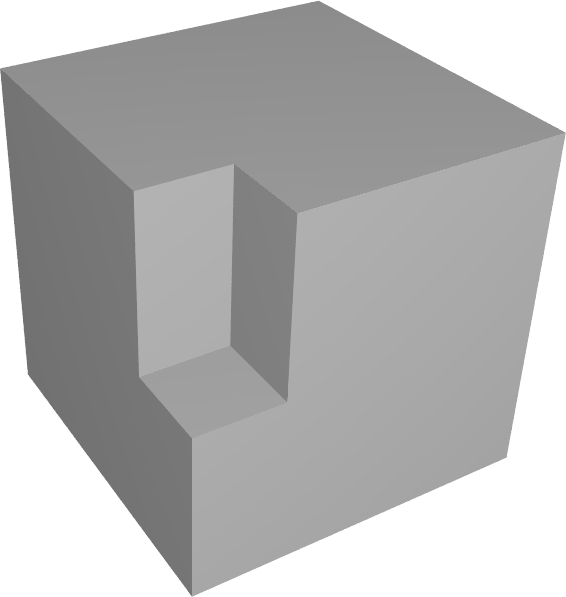
\includegraphics[height=3cm]{boulder.png}\]
\end{uloha}

\eject

\begin{uloha}
Nalezněte všechna reálná řešení soustavy rovnic
\begin{align*}
x^2 + 2y^2 &= 12,\\
x - y &= 3.
\end{align*}
\end{uloha}

\vfil

\begin{uloha}
Je dána rovnice
\[ x^2 - 2 d x + 2 d^2 - 9 = 0 \]
s neznámou $x$ a reálným parametrem $d$. Určete všechny hodnoty $d$, pro které rovnice nemá v reálných číslech řešení.
\end{uloha}


\end{document}